\documentclass[final, 9pt, svgnames, xcolor=table]{beamerPerdy}
\usetheme[
    titleformat title=smallcaps,
    progressbar=frametitle,
    numbering=fraction
]{metropolis}

% Use Fira Sans to improve readability
\setsansfont[BoldFont={Fira Sans SemiBold}]{Fira Sans Book}

\definecolor{Teal}{HTML}{008080}

\usetikzlibrary{positioning,fit,arrows.meta}

%\setbeameroption{show notes on second screen=right}

\setdefaultlanguage{english}

% Comando para usar comentarios
\newcommand{\comment}[1]{\textcolor{comment}{\footnotesize{#1}\normalsize}}

\newcommand\ImageNode[3][]{
    \node[draw=mLightBrown,line width=1pt,#1] (#2) {\includegraphics[width=1cm,height=1cm]{#3}};
}


\title{Validation of Machine Learning services}
\subtitle{Do not let your Machine Learning service going into production without being tested}
\author[J. A. Perdiguero López]{
José Antonio Perdiguero López\\
\href{http://www.perdy.io}{\scriptsize{\faGlobe\; http://www.perdy.io}}\\
\href{https://github.com/perdy}{\scriptsize{\faGithub\; https://github.com/perdy}}\\
\href{https://www.linkedin.com/in/perdy}{\scriptsize{\faLinkedin\; https://www.linkedin.com/in/perdy}}\\
\href{mailto://perdy@perdy.io}{\scriptsize{\faAt\; perdy@perdy.io}}}
\institute[Piksel]{Software Architect @ Piksel}
\date{May 20, 2019}

\begin{document}

% Title
\begin{frame}[noframenumbering, plain]
    \titlepage
\end{frame}

% Index
\begin{frame}[noframenumbering, plain]{Index}
    \setbeamertemplate{section in toc}[circle]
    \tableofcontents
\end{frame}

% Introduction 
\section{Introduction}
\begin{frame}{Introduction}
    What's wrong with current API frameworks? Nothing at all, except they seems a bit \textbf{old} and \textbf{unexpressive}.

    Let's improve it using new Python functionalities like:
    
    \begin{itemize}
        \item Type annotation.
        \item Module \texttt{typing}. 
        \item New \texttt{async}/\texttt{await} semantic.
        \item Module \texttt{asyncio}.
    \end{itemize}
\end{frame}

\begin{frame}{Introduction}
    The codebase can be very \textbf{expressive} in terms of describing the API. Make it the first information source of the API.
\end{frame}

\begin{frame}{Goals}
    \textbf{Speep up} API building and maintenance.

    Create an API with a codebase \textbf{expressive}.

    An \textbf{interactive documentation} kept \textbf{in sync} with the API.

    A way to infer and generate API \textbf{schema}.

    Possibility to work with \textbf{ASGI} and \textbf{websockets}.
\end{frame}

\begin{frame}{Example API}
    Puppy API \faPaw

    \begin{itemize}
        \item \textbf{Register} a new puppy.
        \item \textbf{List} all puppies, filtered by name.
    \end{itemize}
\end{frame}

\begin{frame}[fragile]{Example API}
    \begin{minted}[fontsize=\footnotesize]{python}
def puppy(request):
    if request.method == "POST":
        data = JSONParser().parse(request)
        serializer = PuppySerializer(data=data)
        if serializer.is_valid():
            serializer.save()
            return JsonResponse(serializer.data, status=201)
        return JsonResponse(serializer.errors, status=400)

    if request.method == "GET":
        puppies = Puppy.objects.all()
        name = request.query_params.get('name', None)
        if name is not None:
            puppies = puppies.filter(name=name)
        serializer = PuppySerializer(puppies, many=True)
        return JsonResponse(serializer.data, safe=False)
    \end{minted}
\end{frame}

% Machine Learning 
\section{Machine Learning}
\begin{frame}{What is Artificial Intelligence?}
    Artificial intelligence is the simulation of human intelligence processes by computer systems. These processes include \textbf{learning} (the acquisition of information and rules for using the information), \textbf{reasoning} (using rules to reach approximate or definite conclusions) and \textbf{self-correction}.

    \pause

    AI can be categorized as either \textbf{weak} or \textbf{strong}.

    \pause

    \begin{block}{Strong AI}
		Also known as artificial general intelligence. Is an AI system with generalized human cognitive abilities. When presented with an unfamiliar task, a strong AI system is able to find a solution without human intervention.
    \end{block}

    \pause

    \begin{block}{Weak AI}
		Also known as narrow AI. Is an AI system that is designed and trained for a particular task.
    \end{block}
\end{frame}

\begin{frame}{AI in perspective}
    \only<1>{
        \begin{figure}
            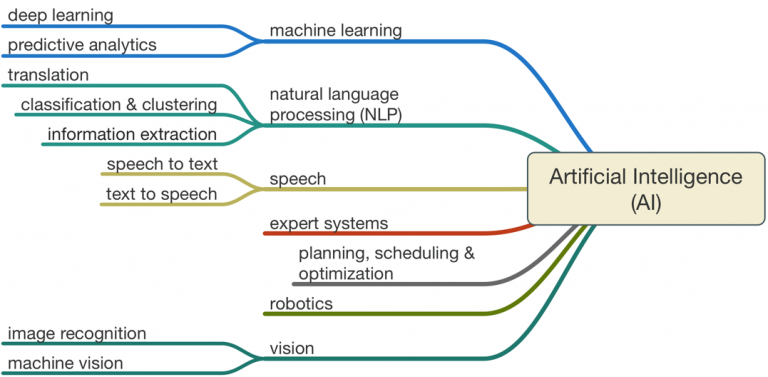
\includegraphics[width=\textwidth]{img/tree-ai.png}
        \end{figure}
    }

    \only<2>{
        \begin{figure}
            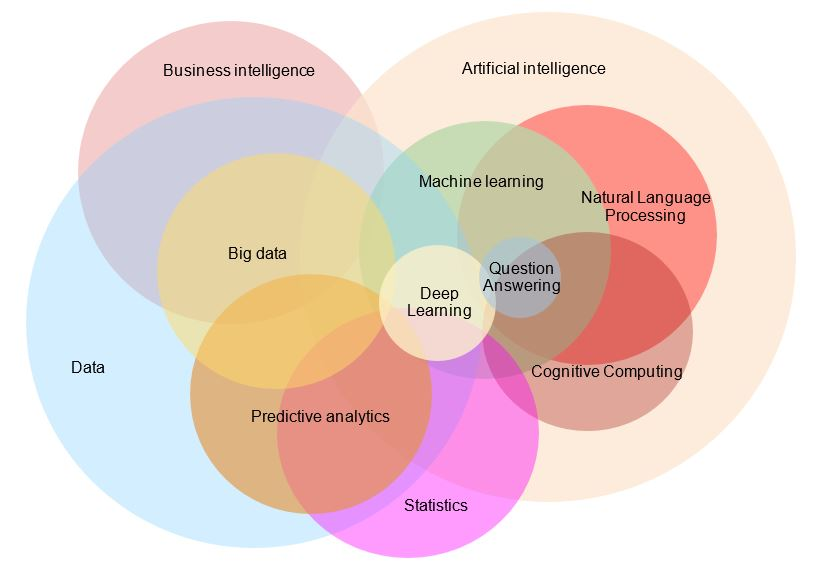
\includegraphics[width=\textwidth]{img/venn-ai.jpeg}
        \end{figure}
    }

    \only<3>{
        \begin{figure}
            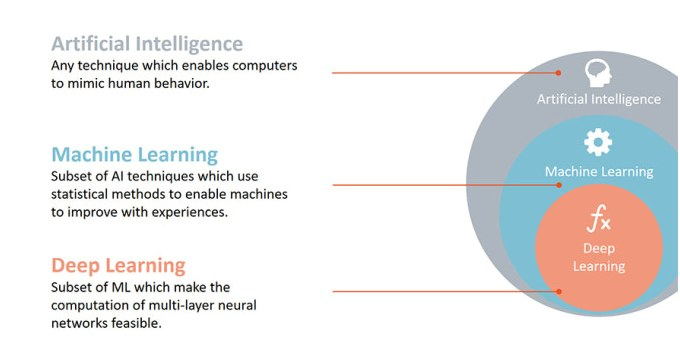
\includegraphics[width=\textwidth]{img/venn-ai-simplified.jpeg}
        \end{figure}
    }
\end{frame}

\begin{frame}{What is Machine Learning?}
    The science of getting a computer to act without programming. There are three types of machine learning algorithms:

    \pause

    \begin{block}{Supervised learning}
        Data sets are labeled so that patterns can be detected and used to label new data sets.
    \end{block}

    \pause

    \begin{block}{Unsupervised learning}
        Data sets aren't labeled and are sorted according to similarities or differences.
    \end{block}

    \pause

    \begin{block}{Reinforcement learning}
        Data sets aren't labeled but, after performing an action or several actions, the AI system is given feedback.
    \end{block}
\end{frame}

\begin{frame}{Supervised Learning}
    \begin{figure}
        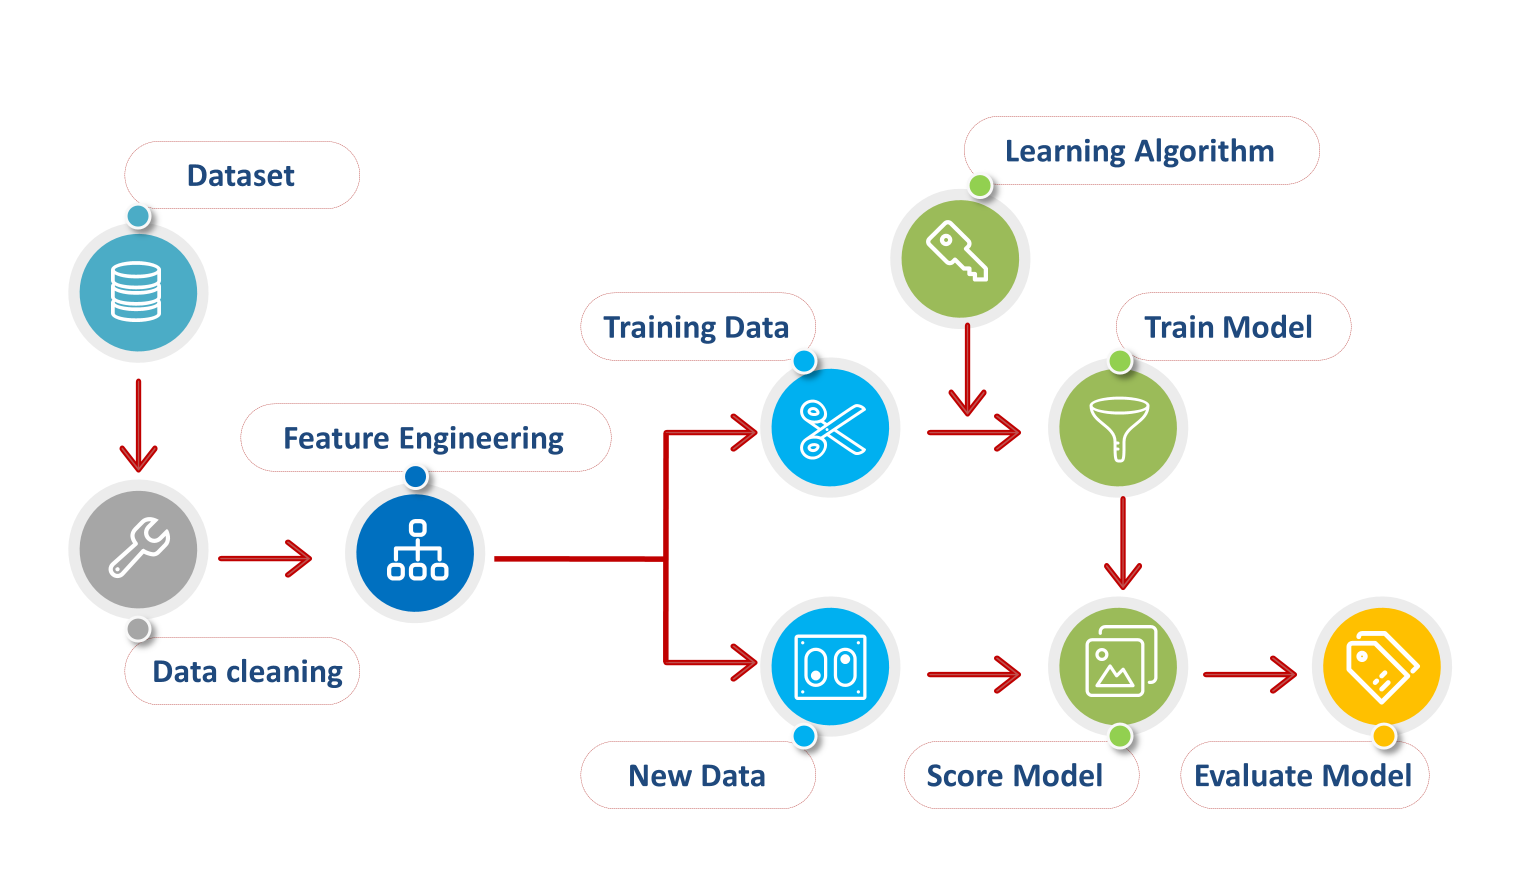
\includegraphics[width=\textwidth]{img/training-process.png}
    \end{figure}
\end{frame}

\begin{frame}{The Model}
    We are going to build a model that performs a sentiment analysis over a text and concludes if it is positive or negative.

    \textbf{Input:} A text (a list of integers representing each word).

    \textbf{Output:} 0 (negative) or 1 (positive).

    \begin{figure}
        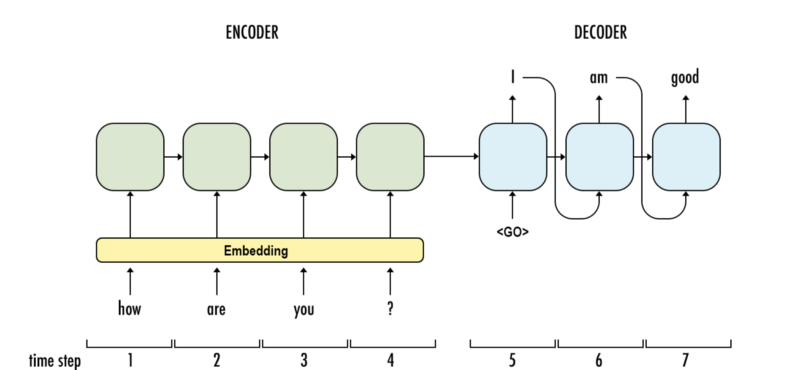
\includegraphics[width=\textwidth]{img/lstm-model.png}
    \end{figure}
\end{frame}

\begin{frame}{Training Dataset}
    The dataset used for training this model is based on movie's reviews from IMDB.

    \qquad

    \rowcolors{1}{}{gray!20}
    \begin{tabular}{lcc}
        \toprule
        \multicolumn{1}{c}{\textbf{Text input}} & \textbf{Input} & \textbf{Output} \\
        \midrule
        the as you with out themselves... & [1, 14, 22, 16, 43, 530, ...] & 1 \\
        the thought solid thought sena... & [1, 194, 1153, 194, 8255, ...] & 0 \\
        the as there in at by br of su... & [1, 14, 47, 8, 30, 31, 7, ...] & 0 \\
        the of bernadette mon they hal... & [1, 4, 18609, 16085, 33, ...] & 1 \\
        the sure themes br only acting... & [1, 249, 1323, 7, 61, 113, ...] & 0 \\
        \bottomrule
    \end{tabular}
\end{frame}

% Building a Machine Learning Service
\section{Building a Machine Learning Service}
\begin{frame}{How to expose the ML model?}
    Machine Learning models can be used either as an internal piece of a service or as a service itself.

    \pause

    If it is used as an \textbf{internal piece} you won't notice it, such as scoring or recommendation systems within bigger products like Spotify or Netflix.

    \pause

    But you can also find them as a \textbf{service that exposes an API} to directly interact with the model. There are many examples of that in AWS, Google Cloud, Azure...
\end{frame}

\begin{frame}{Wrapping up a ML model}
    One of the most widely adopted way of serving a ML model is to wrap it into a \textbf{REST API} with specific methods for calling the model.
\end{frame}

\begin{frame}[fragile]{The Service}
    Our service will expose a single endpoint that let us interact with the model.

    \begin{exampleblock}{Request}
        {
            \footnotesize
            \begin{description}
                \item[Verb] \texttt{\textbf{GET}}
                \item[URL] \texttt{https://service.url/analyze/}
                \item[Params] \texttt{text=The\%20girl\%20is\%20having\%20fun\%20while\%20playing}
            \end{description}
        }
    \end{exampleblock}

    \begin{exampleblock}{Response}
        \begin{minted}[fontsize=\footnotesize]{js}
{
  "text": "The girl is having fun while playing",
  "sentiment": "Positive",
  "score": 0.6321590542793274
}
        \end{minted}
    \end{exampleblock}
\end{frame}

\begin{frame}{Building a REST API with Flama}
    To build a REST API we need to define:

    \begin{enumerate}[<+->]
        \item A \textbf{component} that loads our ML model.
        \item The \textbf{data schema} for our response.
        \item The \textbf{view} function that will be called through requests to \texttt{/analyze/} endpoint.
        \item The whole API \textbf{application}.
    \end{enumerate}

    \only<4>{
        Everything put together is less than 100 lines of python code.
    }
\end{frame}

\begin{frame}[fragile]{ML Component}
    \begin{minted}[fontsize=\footnotesize]{python}
class SentimentAnalysisModel:
    def __init__(self, model, words: typing.Dict[str, int]):
        self.model = model
        self.words = words

    def predict(self, text: str) -> typing.Tuple[float, str]:
        x = text.lower().split()
        x = [self.words.get(i, 0)
             if self.words.get(i, 0) <= VOCABULARY_LENGTH else 0 for i in x]
        x = sequence.pad_sequences([x], maxlen=MAX_WORDS)
        score = self.model.predict(x)
        sentiment = "Positive" if self.model.predict_classes(x)[0][0] == 1 \
            else "Negative"

        return score, sentiment

class SentimentAnalysisModelComponent(Component):
    def __init__(self, model_path: str, words_path: str):
        self.model = load_model(model_path)
        self.model._make_predict_function()
        with open(words_path) as f:
            self.words = json.load(f)

    def resolve(self) -> SentimentAnalysisModel:
        return SentimentAnalysisModel(model=self.model, words=self.words)
    \end{minted}
\end{frame}

\begin{frame}[fragile]{Data Schema}
    \begin{minted}[fontsize=\footnotesize]{python}
class SentimentAnalysis(Schema):
    text = fields.String(
        title="text",
        description="Text to analyze"
    )
    score = fields.Float(
        title="score",
        description="Sentiment score in range [0,1]"
    )
    sentiment = fields.String(
        title="sentiment",
        description="Sentiment class (Positive or Negative)"
    )
    \end{minted}
\end{frame}

\begin{frame}[fragile]{Analysis View}
    \begin{minted}[fontsize=\footnotesize]{python}
def analyze(text: str, model: SentimentAnalysisModel) -> SentimentAnalysis:
    """
    tags:
        - sentiment-analysis
    summary:
        Sentiment analysis.
    description:
        Performs a sentiment analysis on a given text.
    responses:
        200:
            description: Analysis result.
    """
    text = unquote(text)
    score, sentiment = model.predict(text)

    return {
        "text": text,
        "score": score,
        "sentiment": sentiment,
    }
    \end{minted}
\end{frame}

\begin{frame}[fragile]{API Application}
    \begin{minted}[fontsize=\footnotesize]{python}
app = Flama(
    components=[SentimentAnalysisModelComponent("model.h5", "words.json")],
    title="Sentiment Analysis",
    version="0.1",
    description="A sentiment analysis API for movies reviews",
)

app.add_route("/analyze/", analyze, methods=["GET"])
    \end{minted}
\end{frame}

% Testing the service
\section{Testing the Service}
\begin{frame}{Testing Considerations}
    The most commons development cases of Machine Learning services are those where the building of the model and the service are done completely separated and even by different teams.

    That implies we aren't in control of the training process so that we cannot test the model until both are merged.
\end{frame}

\begin{frame}{Validation vs Verification}
    \rowcolors{1}{}{gray!20}
    \begin{tabular}{lp{1.6in}p{1.6in}}
        \toprule
        \textbf{Criteria} & \textbf{Verification} & \textbf{Validation} \\
        \midrule
        \emph{Definition} & The process of evaluating products of a development phase to determine whether they meet the specified requirements. & The process of evaluating software during or at the end of the development process to determine whether it satisfies specified business requirements. \\
        \emph{Objective} & To ensure that the product is being built according to the requirements and design specifications. & To demonstrate that the product fulfills its intended use when placed in its intended environment. \\
        \emph{Question} & Are we building the product right? & Are we building the right product? \\
        \bottomrule
    \end{tabular}
\end{frame}

\begin{frame}[fragile]{Test Specification: Verification}
    \footnotesize{
        \begin{verbatim}
## Endpoint Verification
Tags: functional, verification

Verify if the endpoint that allows interaction with Sentiment Analyzer
is properly defined based on specifications. It must provide a query
parameter **text** that acts as the input of the model and it cannot be
empty. The response must be a JSON containing three attributes:
**text**, **score** and **sentiment**.

* Request sentiment analysis with text "Perdy is testing this" returns "200"
* Response schema contains attributes
    |Attribute|
    |---------|
    |text     |
    |score    |
    |sentiment|
* Request sentiment analysis with text "" returns "400"
        \end{verbatim}
    }
\end{frame}

\begin{frame}[fragile]{Test Specification: Validation}
    \footnotesize{
        \begin{verbatim}
## Model Validation
Tags: ml, validation

Validate the model predictions against a set of fixed data. This data set
must contains a minimum list of well-known pairs of input and output to
check that after retraining the model it will continue behaving the same
way against these inputs.

* Analyze and validate the following texts <table:data/sentiment_analysis.csv>
        \end{verbatim}
    }
\end{frame}

\begin{frame}[fragile]{Step Implementation}
    \begin{minted}[fontsize=\footnotesize]{python}
@step("Response schema contains attributes <table>")
def assert_response_schema(table):
    response = data_store.scenario["response"]

    for attribute in table.get_column_values_with_name("Attribute"):
        assert attribute in response
    \end{minted}
\end{frame}

\begin{frame}{Console Output}
    \begin{figure}
        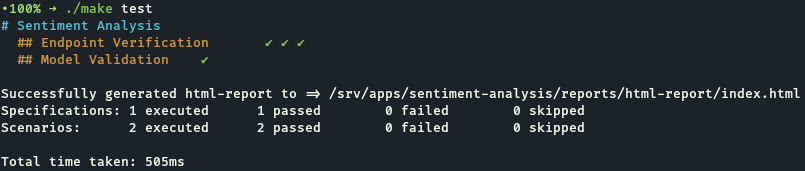
\includegraphics[width=\textwidth]{img/test-console-output.png}
    \end{figure}
\end{frame}

\begin{frame}{HTML Output}
    \begin{figure}
        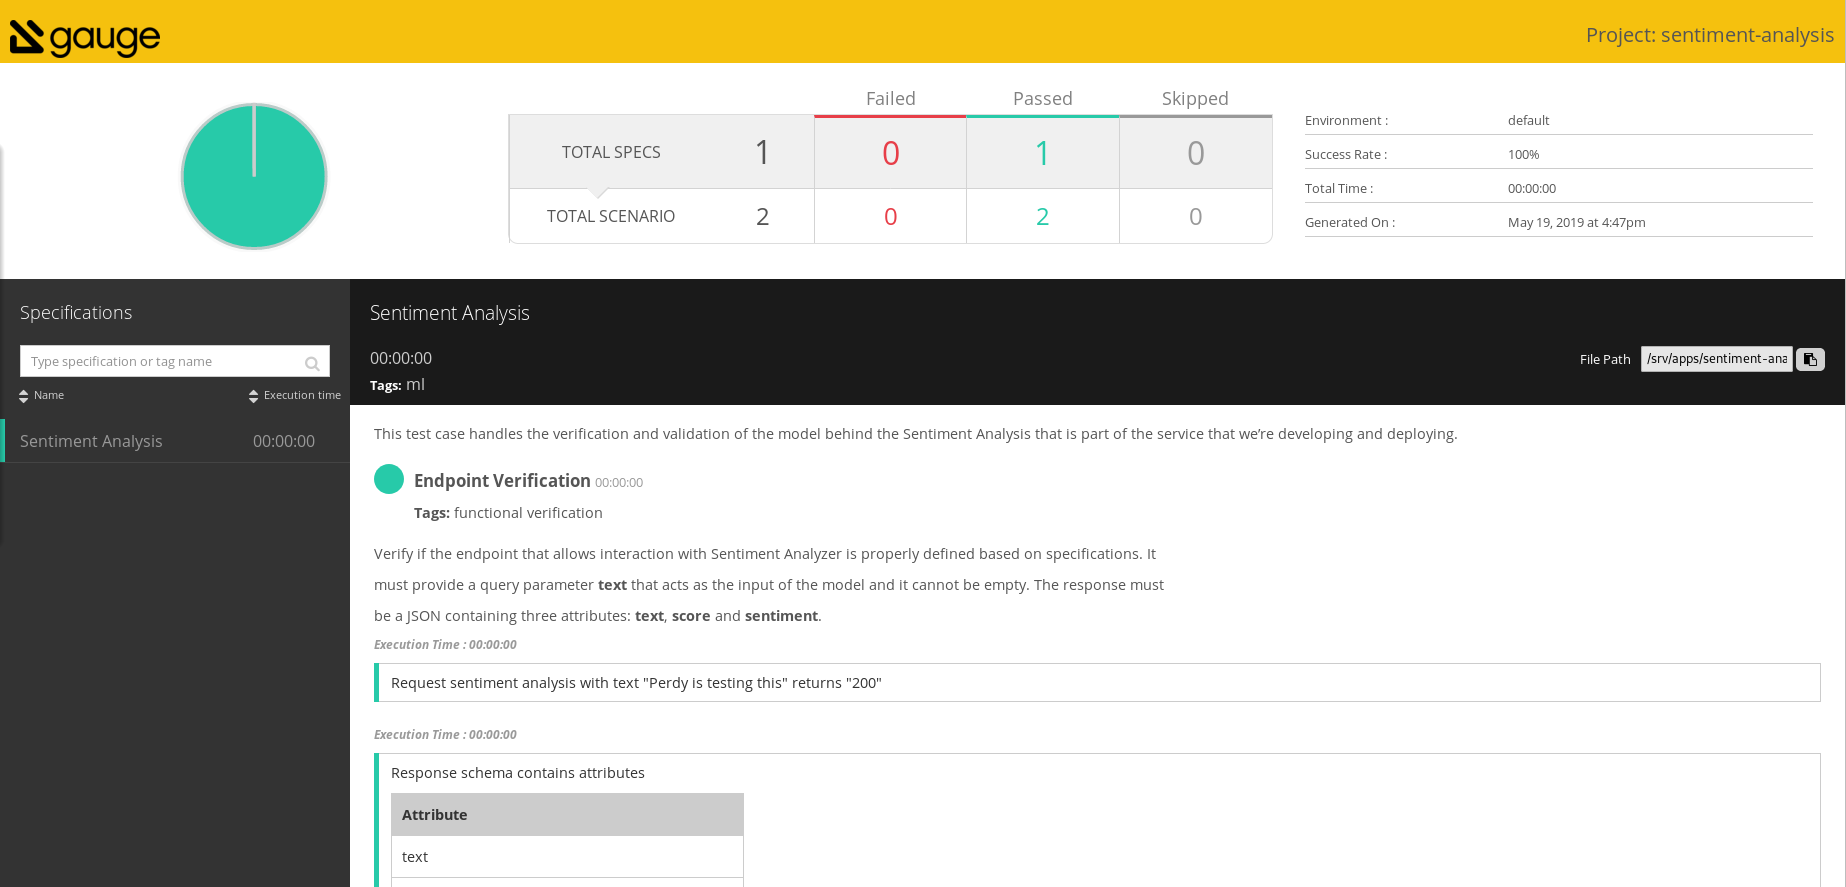
\includegraphics[width=\textwidth]{img/test-html-output.png}
    \end{figure}
\end{frame}


\begin{frame}[standout]
    \Huge{Support open source projects: \\ \faStar \, Give a star\\ \faBullhorn \, Spread the word}

    \qquad

    \href{https://flama.perdy.io}{https://flama.perdy.io/}

    \href{https://getgauge.io/}{https://getgauge.io/}

    \href{https://www.tensorflow.org/}{https://www.tensorflow.org}

    \href{https://www.python.org/}{https://www.python.org/}
\end{frame}

\end{document}
